%%%%% Don't Make Changes Below Here %%%%%
\documentclass{article}\usepackage[utf8]{inputenc}\usepackage[margin=0.4cm,top=0.4cm,bottom=0.4cm]{geometry}\usepackage[usenames,dvipsnames,svgnames,table]{xcolor}\usepackage{bm, multicol}\usepackage{calligra}\usepackage{tikz, listings}\usepackage{hyperref}\usetikzlibrary{matrix,fit,chains,calc,scopes}\usepackage{tcolorbox}\tcbuselibrary{skins}\tcbset{Baystyle/.style={sharp corners,enhanced,boxrule=6pt,colframe=orange,height=\textheight,width=\textwidth,borderline={8pt}{-11pt}{},}}\usepackage{amsmath,amssymb,amsthm,tikz,tkz-graph,color,chngpage,soul,hyperref,csquotes,graphicx,floatrow}\newcommand*{\QEDB}{\hfill\ensuremath{\square}}\newtheorem*{prop}{Proposition}\renewcommand{\theenumi}{\alph{enumi}}\usepackage[shortlabels]{enumitem}\usetikzlibrary{matrix,calc}\MakeOuterQuote{"}\newtheorem{theorem}{Theorem} \usetikzlibrary{shapes} \usepackage{lipsum}\usepackage{tabularx,ragged2e,booktabs,caption}\tcbuselibrary{breakable}\newenvironment{yframed}{\begin{tcolorbox}[breakable,colback=gray!3,title after break={\textit{\color{red}Solution (cont.)}},colbacktitle=gray!3, coltitle=black,titlerule=-1pt] }{\end{tcolorbox}}\newtcolorbox{mybox}{colback=black!15!white, colframe=white,arc=12pt}\newtcolorbox{myboxot}{colback=green!15!white, colframe=white,arc=12pt,width=110pt, height=27pt}\newtcbox{\mylib}{enhanced,boxrule=0pt,top=0mm,bottom=0mm,right=0mm,left=4mm,arc=4pt,boxsep=9pt,before upper={\vphantom{dlg}},colframe=green!50!black,coltext=green!25!black,colback=green!10!white,overlay={\begin{tcbclipinterior}\fill[green!75!blue!50!white] (frame.south west)rectangle node[text=white,font=\sffamily\bfseries\tiny,rotate=90] {Problem} ([xshift=4mm]frame.north west);\end{tcbclipinterior}}}\newtcbox{\mylibot}{enhanced,boxrule=0pt,top=0mm,bottom=0mm,right=0mm,arc=4pt,boxsep=9pt,before upper={\vphantom{dlg}},colframe=green!50!black,coltext=green!25!black,colback=green!10!white,overlay={\begin{tcbclipinterior}\fill[red!75!blue!50!white] (frame.south west)rectangle node[text=white,font=\sffamily\bfseries\tiny,rotate=90] {Other} ([xshift=4mm]frame.north west);\end{tcbclipinterior}}}
\def\Title{\begin{tcolorbox}[Baystyle,]{\begin{center}\vspace*{0.14\textheight}
{\rule{\textwidth}{1.6pt}\vspace*{-\baselineskip}\vspace*{2pt}}
\rule{\textwidth}{0.4pt}\\[0.2\baselineskip]{\fontsize{45}{45}\scshape CS 189: Introduction to Machine Learning \\[0.2\baselineskip] \calligra Spring 2018 \\[0.2\baselineskip]}
{\rule{\textwidth}{0.4pt}\vspace*{-\baselineskip}\vspace{3.2pt}}
\rule{\textwidth}{1.6pt}\\[\baselineskip]\vspace{0.05\textheight}{{\fontsize{45}{45}\scshape$\bullet$\\ {Homework 6}\\\vspace*{0.01\textheight} }{{\fontsize{18}{18}\scshape{Due on Sunday, March 4th, 2018 at 10pm\\}}}\fontsize{45}{45}\scshape$\bullet$  \\}\vspace*{0.1\textheight}{\fontsize{12}{12}\calligra Solutions by\\}{\fontsize{28}{28}\scshape \Name \\}\vspace*{0.01\textheight}{\fontsize{12}{12}\scshape \SID} \\\vspace*{0.05\textheight}{\fontsize{12}{12}\calligra In collaboration with\\}\vspace*{0.01\textheight}{\fontsize{12}{12}\scshape \Collabs} \\\vspace*{0.05\textheight}\end{center}}\end{tcolorbox}\newgeometry{margin=0.75in}}\def\BeginSolution{\begin{yframed}\textbf{\color{red}Solution }}\def\EndSolution{\end{yframed}}\usepackage{algorithm}\usepackage[noend]{algpseudocode}\makeatletter\def\BState{\State\hskip-\ALG@thistlm}\makeatother\def\star{\bigstar}\usetikzlibrary{arrows}\usepackage[mathscr]{euscript}\usepackage[T1]{fontenc}\DeclareSymbolFont{rsfs}{U}{rsfs}{m}{n}\DeclareSymbolFontAlphabet{\mathscrsfs}{rsfs}\newcommand\tab[1][1cm]{\hspace*{#1}}\hypersetup{colorlinks=true,urlcolor=blue}\newtheorem{lemma}[theorem]{Lemma}\newcommand{\norm}[1]{\left\lVert#1\right\rVert}\def\vec{\mathbf}\def\y{\mathbf{y}}\def\X{\mathbf{X}}\def\R{\mathbb{R}}\def\x{\mathbf{x}}\def\w{\mathbf{w}}\def\T{^\top}\def\r{\mathbf{r}}\def\mat{\mathbf}\def\I{\mathbf{I}}\def\A{\mathbf{A}}\newcommand{\num}{n}\newcommand{\dims}{d}\def\real{\mathbb{R}}\def\ev{\mathbb{E}}\newcommand{\whatridge}{\widehat{w}_\lambda}\def\calN{\mathcal{N}}\newcommand{\hatwPCA}{\vec{\widehat{w}}_\text{{PCA}}}\newcommand{\hatyPCA}{\vec{\widehat{y}}_{\text{PCA}}}\newcommand{\hatwOLS}{\vec{\widehat{w}}_{\text{OLS}}}\newcommand{\hatwridge}{\vec{\widehat{w}}_{\text{ridge}}}\newcommand{\tildewridge}{\vec{\tilde{w}}_{\text{ridge}}}\newcommand{\hatyridge}{\vec{\hat{y}}_{\text{ridge}}}\def\diag{\operatorname{diag}}\newcommand*\circled[1]{\tikz[baseline=(char.base)]{\node[circle,fill=white!20,draw,inner sep=1pt,opacity=1,text opacity=0] (char) {#1};}}\newcommand\citem{\item[\circled{\Alph{enumi}}]}
%%%%% Don't Make Changes Above Here %%%%%

%%%%% Template Begins Here %%%%%

\def\Name{Firstname Lastname}  % Your name
\def\SID{Student ID}  % Your student ID number
\def\Collabs{None} % Your collaborators here with a comma between each person's name. Write None if no collaborators. Don't leave blank.


\pagestyle{empty}
\begin{document}
\Title
\clearpage

%%%% Problem 1 Starts Here %%%%
\vspace{-2mm}\noindent\begin{mybox}{\begin{center}\textbf{\color{black}Problem 1: Getting Started}\end{center}}\end{mybox}\vspace{-2mm}
\vspace{10pt}
\noindent \textbf{Read through this page carefully.} You may typeset your homework in latex or submit neatly handwritten/scanned solutions. Please start each question on a new page. Deliverables:
\begin{enumerate}[1.]
\item Submit a PDF of your writeup, \textbf{with an appendix for your code}, to assignment on Gradescope, ``HW6 Write-Up''. If there are graphs, include those graphs in the correct sections. Do not simply reference your appendix.
\item If there is code, submit all code needed to reproduce your results, ``HW6 Code''.
\item If there is a test set, submit your test set evaluation results, ``HW6 Test Set''.
\end{enumerate}
After you've submitted your homework, watch out for the self-grade form.
\begin{enumerate}
\item Who else did you you work with on this homework? In case of course events, just describe the group. How did you work on this homework? Any comments about the homework?
\BeginSolution
%1a

\EndSolution
\item Please copy the following statement and sign next to it. We just want to make it \textit{extra} clear so that no one inadvertently cheats.

\textit{I certify that all solutions are entirely in my words and that I have not looked at another student's solutions. I have credited all external sources in this write up.}
\BeginSolution
%1b

\EndSolution
\end{enumerate}
%%%% Problem 1 Ends Here %%%%
\clearpage

%%%% Problem 2 Starts Here %%%%
\vspace{-2mm}\noindent\begin{mybox}{\begin{center}\textbf{\color{black}Problem 2: Canonical Correlation Analysis}\end{center}}\end{mybox}\vspace{-2mm}
\vspace{10pt}
\noindent The goal of canonical correlation analysis (CCA) is to find linear combinations that maximize the correlation of two random vectors. We are given two zero-mean random vectors $\vec X, \vec Y \in \mathbb{R}^d$. Any linear combination of the coordinates of the random vector $\vec X$ can be written as $\vec{a}^\top \vec X$, and similarly, a linear combination of the coordinates of the random vector $\vec Y$ can be written as $\vec{b}^\top \vec Y$. Note that $\vec{a}^\top \vec X, \vec{b}^\top \vec Y \in \mathbb{R}$ are scalar random variables.
\vspace{4pt}

\noindent The goal of CCA can be summarized as solving the following optimization problem \begin{equation} \rho = \max_{\vec{a}, \vec{b} \in \mathbb{R}^d} \rho(\vec{a}^\top \vec X, \vec{b}^\top \vec Y). \end{equation} where  the correlation coefficient $\rho(P, Q)$ between two zero-mean scalar random variables $P$ and $Q$ is defined by \begin{align*} \rho(P, Q) = \frac{\ev [PQ]}{\sqrt{\ev[P^2] \ev[Q^2]}}. \end{align*} The zero-mean jointly-Gaussian case expresses why we care about correlation. Two jointly Gaussian zero-mean random variables that are uncorrelated are also independent of each other. Furthermore, if we want to best estimate (in a mean-squared sense) a particular scalar zero Gaussian random variable $Y$ based on a vector $\vec X$ of jointly Gaussian zero-men random variables, then we are going to pick a weight vector $\vec{w}$ that is aligned with $\ev[\vec X Y]$. It is straightforward algebra to see that this direction maximizes the correlation coefficient $\rho (\frac{\vec{w}^{\top}}{\| \vec w |} \vec X, Y)$.
\vspace{4pt}

\noindent In this problem, we will work our way towards finding a solution to the problem of canonical correlation analysis using the singular value decomposition. In parts (a) to (c), we derive useful results regarding the singular value decomposition. In the later parts, you will use this result and see that canonical correlation analysis is equivalent to the singular value decomposition in a rotated and stretched coordinate system.
\begin{enumerate}
\item Let $n \geq d$. For a matrix $\mat{A} \in \mathbb{R}^{n \times d}$ with full column-rank and singular value decomposition $\mat{A} = \mat{U} \mat \Sigma \mat{V}^\top$, we know that the singular values are given by the diagonal entries of $\mat \Sigma$, and the left singular vectors are the columns of the matrix $\mat{U}$ and the right singular vectors are the columns of the matrix $\mat{V}$. Note that both the matrices $\mat{U}$ and $\mat{V}$ have orthonormal columns.
\vspace{4pt}

\noindent {\bf Show that $\mat{A} = \sum_{i=1}^d \sigma_i \vec{u}_i \vec{v}_i^\top$, where the $i$th singular value is denoted by $\sigma_i = \mat \Sigma_{ii}$ and $\vec{u}_i$ and $\vec{v}_i$ are the $i$th left and right singular vectors, respectively.}
\BeginSolution
%2a

\EndSolution
\item {\bf With the setup above, show that}
\begin{enumerate}[i.]
\item {\bf $\mat{A}^\top \mat{A}$ has $i$-th eigenvalue $\sigma_i^2$, with associated eigenvector $\vec{v}_i$.}
\BeginSolution
%2bi

\EndSolution
\item {\bf $\mat{A} \mat{A}^\top$ has $i$-th eigenvalue $\sigma_i^2$, with associated eigenvector $\vec{u}_i$.}
\BeginSolution
%2bii

\EndSolution
\end{enumerate}
Notice that both of the above matrices are symmetric.
\item {\bf Use the first part to show that \begin{align*} \sigma_1 (\mat{A}) = \max_{\substack{\vec{u}: \|\vec{u}\|_2 = 1 \\ \vec{v}: \|\vec{v}\|_2 = 1}} \vec{u}^\top \mat{A} \vec{v}, \end{align*} where $\sigma_1(\mat{A})$ is the maximum singular value of $\mat{A}$.
\vspace{4pt}

\noindent Additionally, show that if $\mat{A}$ has a unique maximum singular value, then the maximizers $(\vec{u}^*, \vec{v}^*)$ above are given by the first left and right singular vectors, respectively.}
\vspace{4pt}

\noindent Hint 1: You may or may not find the following fact useful: We can express any $\vec{u} \in \R^n: \|\vec{u} \|_2 = 1$ as a linear combination of left singular vectors $\{ \vec u_i \}$ of the matrix $\mat{A}$, and any vector $\vec{v} \in \R^d$ as a linear combination of the right singular vectors $\{ \vec v_i \}$ of the matrix $\mat A$.
\vspace{4pt}

\noindent Hint 2: You may find the following results: For any two vectors $\vec{a}, \vec{b} \in \mathbb{R}^d$, we have
\begin{itemize}
\item Cauchy-Schwarz inequality: $|\vec{a}^\top \vec{b}| \leq \|\vec{a}\|_2 \|\vec{b}\|_2$, with equality only when $\vec{b}$ is a scaled version of $\vec{a}$.
\item Holder's inequality: $|\vec{a}^\top \vec{b}| \leq \| \vec{a}\|_1 \|\vec{b}\|_\infty$. Here, the $\ell_1$ and $\ell_\infty$ norms of a vector $\vec v$ are defined by $\|\vec{v}\|_1 = \sum_i |v_i|$, and $\|\vec{v}\|_\infty = \max_i |v_i|$.
\begin{itemize}
\item Let us say the vector $\vec{b}$ is fixed; then one way to achieve equality in the Holder inequality is to have: Let $i$ be such that $|b_i| = \|\vec{b}\|_\infty$. Set $a_i = \|\vec{a}\|_1$, and $a_j = 0$ for all $j \neq i$.
\end{itemize}
\end{itemize}
\BeginSolution
%2c

\EndSolution
\item Let us now look at the canonical correlation analysis problem, where we are given the covariance of two zero-mean random vectors $\vec X, \vec Y \in \mathbb{R}^d$ as follows: \begin{align*} \ev [\mat{X}\mat{X}^\top] = \mat \Sigma_{XX}, \quad \ev [\mat{Y}\mat{Y}^\top] = \mat \Sigma_{YY}, \quad \text{and},\quad \ev [\mat{X}\mat{Y}^\top] = \mat \Sigma_{XY}. \end{align*} The goal is to find two directions/unit-vectors $\vec a $ and $\vec b$ so that the resulting scalar random variables $\vec{a}^{\top} \vec X$ and $\vec{b}^{\top} \vec Y$ have maximal correlation coefficient $\rho(\vec{a}^{\top} \vec X, \vec{b}^{\top} \vec Y)$.
\vspace{4pt}

\noindent {\bf Show that the canonical correlation analysis problem can be rewritten as \begin{align*} \rho = \max_{\vec{a}, \vec{b} \in \mathbb{R}^d} \frac{\vec{a}^\top \mat \Sigma_{XY} \vec{b}} { \left( \vec{a}^\top \mat \Sigma_{XX} \vec{a}\right)^{1/2} \left( \vec{b}^\top \mat \Sigma_{YY} \vec{b}\right)^{1/2} }. \end{align*} Conclude that if $(\vec{a}^*, \vec{b}^*)$ is a maximizer above, then $(\alpha \vec{a}^*, \beta \vec{b}^*)$ is a maximizer for any $\alpha, \beta > 0$.} We see that scaling the vectors $\vec a$ or $\vec b$ does not affect their correlation coefficient.
\BeginSolution
%2d

\EndSolution
\item Let us simplify our optimization problem. Assume that the covariance matrices $\mat \Sigma_{XX}$ and $\mat \Sigma_{YY}$ are full-rank. We choose matrices $\mat \Sigma_{XX}^{-\frac{1}{2}}$, $\mat \Sigma_{YY}^{-\frac{1}{2}}$ to whiten the vectors $\vec X$ and $\vec Y$ respectively. Note that for the vector $\tilde{\vec X} = \mat \Sigma_{XX}^{-\frac{1}{2}} \vec X$, we have \begin{align*}  \ev[\tilde{\vec X} \tilde{\vec X^T} ]  = \ev[(\vec X\mat \Sigma_{XX}^{-\frac{1}{2}})^\top(\vec X\mat \Sigma_{XX}^{-\frac{1}{2}})]   = \mat I \end{align*} One may do a similar computation for the whitened vector $\tilde{\vec Y} = \mat \Sigma_{YY}^{-\frac{1}{2}} \vec Y$, and conclude that its covariance matrix is identity too! Such a whitening step simplifies our computations, both at algebraic and conceptual level.
\vspace{4pt}

\noindent {\bf Rewrite the optimization problem from the previous part, using the aforementioned whitening in the following form}: \begin{align*} \rho = \max_{\substack{\vec{c} : \|\vec{c}\|_2 = 1 \\ \vec{d}: \|\vec{d}\|_2 = 1 }} \vec{c}^\top \mat \Sigma_{XX}^{-1/2}\mat \Sigma_{XY} \mat \Sigma_{YY}^{-1/2} \vec{d}. \end{align*}
\BeginSolution
%2e

\EndSolution
\item Recall that the vectors $(\vec{a}^*, \vec{b}^*)$ denote maximizers in the previous part of the problem. Using the simplification and the above parts {\bf show that}
\vspace{4pt}

\noindent $\rho^2$ is the maximum eigenvalue of the matrix $$\mat \Sigma_{XX}^{-1/2} \mat \Sigma_{XY} \mat \Sigma_{YY}^{-1} \mat \Sigma_{XY}^\top \mat \Sigma_{XX}^{-1/2}.$$
\vspace{4pt}

\noindent Hint: An appropriate change of variables may make your life easier.
\BeginSolution
%2f

\EndSolution
\item Following the previous part's setup, {\bf show that} $\vec{c}^* = \mat \Sigma_{XX}^{1/2} \vec{a}^*$ is an eigenvector corresponding to the maximum eigenvalue of the matrix $$\mat \Sigma_{XX}^{-1/2} \mat \Sigma_{XY} \mat \Sigma_{YY}^{-1} \mat \Sigma_{XY}^\top \mat \Sigma_{XX}^{-1/2}.$$
\BeginSolution
%2g

\EndSolution
\item Following the previous part's setup, {\bf show that} $\vec{d}^* = \mat \Sigma_{YY}^{1/2} \vec{b}^*$ is an eigenvector corresponding to the maximum eigenvalue of the matrix $$\mat \Sigma_{YY}^{-1/2} \mat \Sigma_{XY}^\top \mat \Sigma_{XX}^{-1} \mat \Sigma_{XY} \mat \Sigma_{YY}^{-1/2}.$$
\BeginSolution
%2h

\EndSolution
\item {\bf Argue why such a CCA is not meaningful when the random vectors $\vec X$ and $\vec Y$ are uncorrelated, where by this we mean that ${\sf cov}(X_i, Y_j) = 0$ for all $i, j$.}
\BeginSolution
%2i

\EndSolution
\item Suppose you happen to know that $\vec X$ and $\vec Y^2$ (where a squared-vector $\vec Y^2$ is defined by squaring each entry of the vector $\vec Y$) share a linear relationship, {\bf how could you still use CCA effectively with the given data?}
\BeginSolution
%2j

\EndSolution
\item {\bf Why do you think that understanding CCA is relevant for machine learning?}
\BeginSolution
%2k

\EndSolution
\end{enumerate}
%%%% Problem 2 Ends Here %%%%
\clearpage

%%%% Problem 3 Starts Here %%%%
\vspace{-2mm}\noindent\begin{mybox}{\begin{center}\textbf{\color{black}Problem 3: Mooney Reconstruction}\end{center}}\end{mybox}\vspace{-2mm}
\vspace{10pt}
\noindent In this problem, we will try to restore photos of celebrities from Mooney photos, which are binarized faces. In order to do this, we will leverage a large training set of grayscale faces and Mooney faces. Producing a face reconstruction from a binarized counterpart is a challenging high dimensional problem, but we will show that we can learn to do so from data. In particular, using the power of Canonical Correlation Analysis (CCA), we will reduce the dimensionality of the problem by projecting the data into a subspace where the images are most correlated. 
\vspace{4pt}

\noindent Images are famously redundant and well representable in lower-dimensional subspaces as the eigenfaces example in class showed. However, here our goal is to relate two different kinds of images to each other. Let's see what happens.\begin{figure}[h!]    \begin{center}    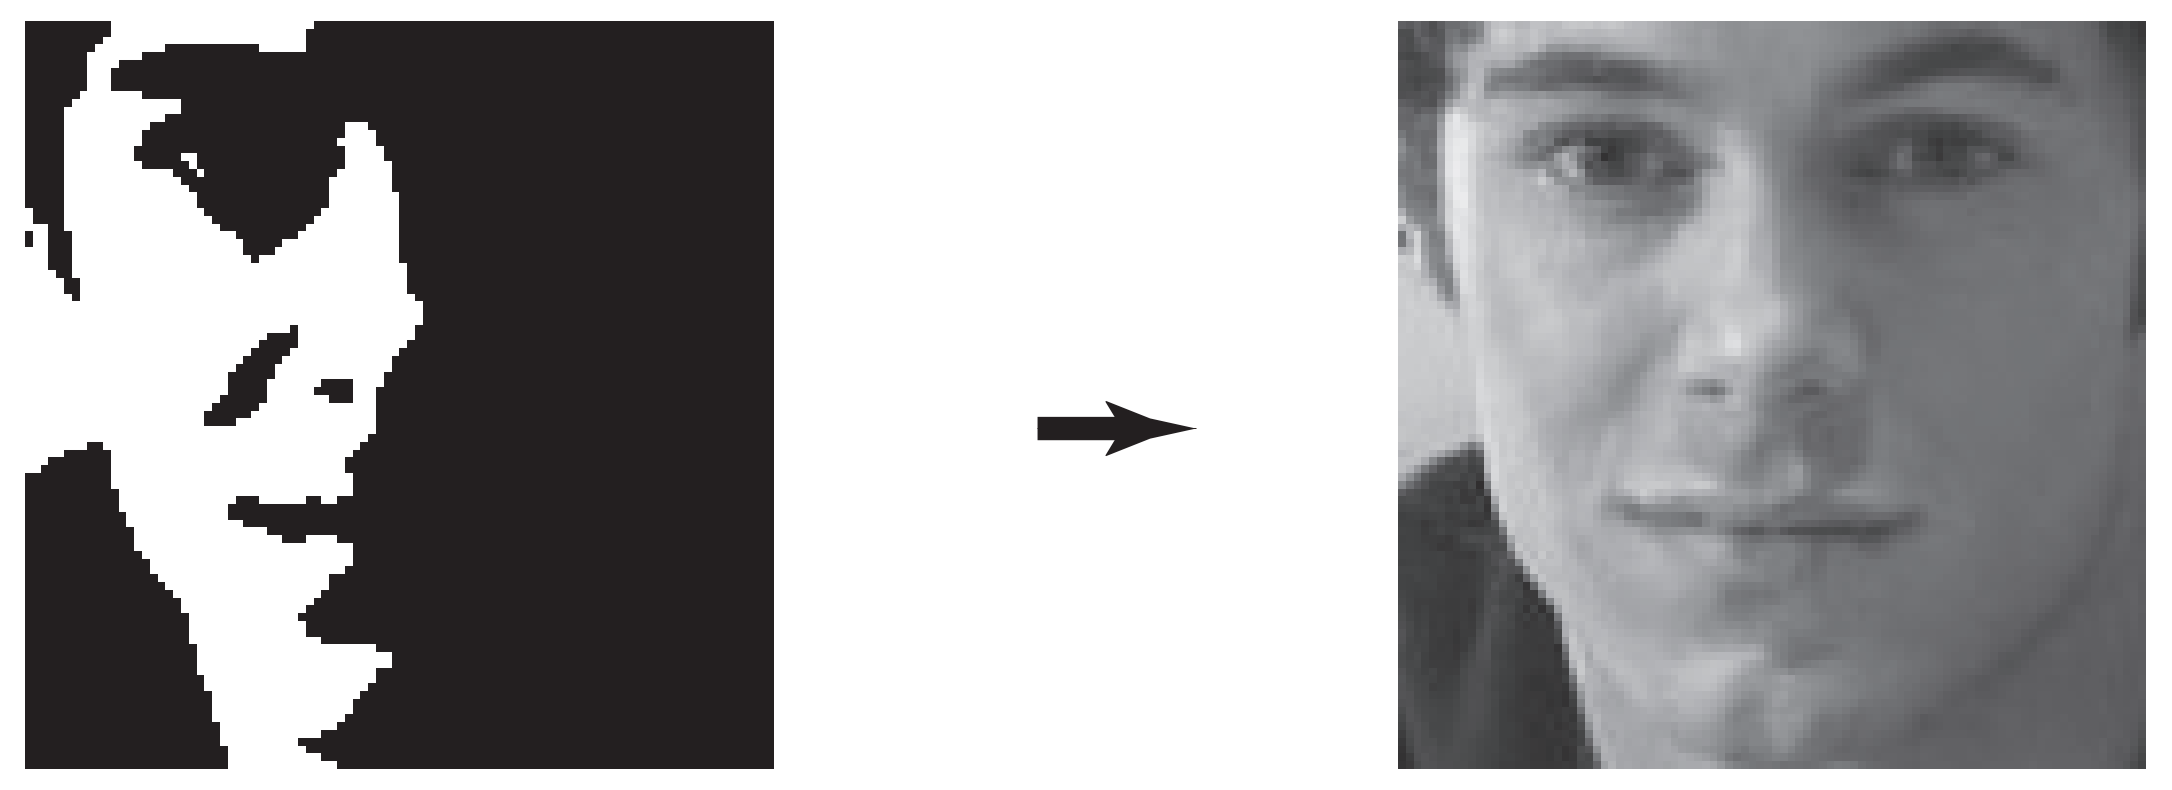
\includegraphics[scale=.4]{images/mooney}    \caption{A binarized Mooney image of an face being restored to its original grayscale image.}    \label{fig:robot}    \end{center}\end{figure} The following datasets will be used for this project: X\_train.p, Y\_train.p, X\_test.p and Y\_test.p. The training data X\_train.p contains 956 binarized images, where each image $\mat X_i \in \mathbb{R}^{15 \times 15   \times 3}$. The test data X\_test.p contains 255 binarized images with the same dimensionality. Y\_train.p contains 956 corresponding grayscale images, where $\mat Y_i \in  \mathbb{R}^{ 15 \times 15 \times 3 }$. Y\_test.p contains 255 grayscale images that correspond to X\_test.p. 
\vspace{4pt}

\noindent Through out the problem we will assume that all data points are flattened and standardize as follows: \begin{align*}	x \mapsto (x/255)*2.0 - 1.0 \quad\text{and}\quad	y \mapsto (y/255)*2.0 - 1.0. \end{align*} {\bf Note} that this standardization step on loading the data does not ensure that the resulting images have zero mean. So removing the mean from the images is an additional processing step.) 
\vspace{4pt}

\noindent Please use only the following libraries to solve the problem in Python 3.0:
\begin{lstlisting}
import pickle
from scipy.linalg import eig
from scipy.linalg import sqrtm
from numpy.linalg import inv
from numpy.linalg import svd
import matplotlib.pyplot as plt
from sklearn.preprocessing import StandardScaler
\end{lstlisting}
\begin{enumerate}
\item We use CCA to find pairs of directions $\vec a$ and $\vec b$ that maximize the correlation between the projections $\tilde{\vec x} = \vec a^T\mathbf{x}$ and $\tilde{y} = \vec b^T\vec{y}$,  From the previous problem, we know that this can be done by solving the problem \begin{align*}	\rho = \max_{\vec a, \vec b} \frac{\vec a^\top \mat \Sigma_{XY} \vec b}{ \left( \vec a^\top \mat \Sigma_{XX} \vec a\right)^{1/2} \left( \vec b^\top \mat \Sigma_{YY} \vec b\right)^{1/2} }, \end{align*} where $\mat \Sigma_{XX}$ and $\mat \Sigma_{YY}$ denote the covariance matrices of the $\mat X$ and $\mat Y$ images, and $\mat \Sigma_{XY}$ denotes the covariance between $\mat X$ and $\mat Y$. Note that unlike in the previous problem, we are not given the covariance matrices and must estimate them from the images samples of $\mat X$ and  $\mat Y$.
\vspace{4pt}

\noindent {\bf Write down how to estimate the three covariance matrices from finite samples of data and implement the code for it}.
\vspace{4pt}

\noindent In order to properly compute the covariance matrices you have to 1) standardize the data, 2) subtract the mean and 3) scale by the number of data points at the end. 
\vspace{4pt}

\noindent Note throughout the homework, we shall use the function StandardScaler to subtract the mean from the data and subsequently add it back. 
\BeginSolution
%3a

\EndSolution
\item We know from the previous problem that we are interested in the maximum singular value of the matrix $\mat \Sigma_{XX}^{-1/2} \mat \Sigma_{XY}\mat \Sigma_{YY}^{-1/2}$, and that this corresponds to the maximum correlation coefficient $\rho$. Now, however, {\bf plot the full ``spectrum'' of singular values of the matrix}  \begin{align*}	(\mat \Sigma_{XX}+\lambda \mat I)^{-1/2} \mat \Sigma_{XY} (\mat \Sigma_{YY}+\lambda \mat I)^{-1/2}. \end{align*} For numerical issues we need to add a very small scalar times the identity matrix to the covariance terms.  Set $\lambda = 0.00001$. 
\BeginSolution
%3b

\EndSolution
\item You should have noticed from the previous part that we have some singular value decay. It therefore makes sense to only consider the top singular value(s), as in CCA. Let us now try to project our images $\mat X$ on to the subspace spanned by the top $k$ singular vectors. Given the SVD $\mat U\mat \Sigma \mat V^T = \mat \Sigma_{XX}^{-1/2} \mat \Sigma_{XY} \mat \Sigma_{YY}^{-1/2}$, we can use the left hand singular vectors to form a projection.  \[ \mat P_k = \begin{bmatrix}   \vec u_0   & \vec u_1 & ... & \vec u_{k-1} \\ \end{bmatrix},   \] {\bf Show/visualize the ``face'' corresponding to the first singular vector $\vec u_0$}. Use the following code for the visualization:
\begin{lstlisting}
	def plot_image(self,vector):
		vector = ((vector+1.0)/2.0)*255.0

		vector = np.reshape(vector,(15,15,3))

		p = vector.astype("uint8")

		p = cv2.resize(p,(100,100))
		count = 0

		cv2.imwrite('singular_face.png',p)
\end{lstlisting}
\BeginSolution
%3c

\EndSolution
\item We will now examine how well the projected data helps generalization when performing regression. You can think of CCA as a technique to help learn better features for the problem. We will use ridge regression regression to learn a mapping, $\mat W \in \mathbb{R}^{k\times 675}$ ($15*15*3=675$), from the projected binarized data to the grayscale images. The binarized images are placed in matrix $\mat X \in \mathbb{R}^{956 \times 675}$\begin{align*}	\underset{\mat W}{\mbox{min}} ||(\mat X\mat P_k) \mat W - \mat Y||^2_2 + \lambda||\mat W||^2_{F}.\end{align*} {\bf Implement Ridge Regression with $\lambda = 0.00001$. Plot the Squared Euclidean test error for the following values of $k$ (the dimensions you reduce to):
\vspace{4pt}

\noindent $k = \lbrace 0,50,100,150,200,250,300,350,400,450,500,650 \rbrace$.}
\BeginSolution
%3d

\EndSolution
\item {\bf Try running the learned model on 4 of the images in the test set and report the results. Give both the binarized input, the true grayscale, and the output of your model.} You may use the code from previous part to visualize the images. \begin{figure}[h!]    \begin{center}    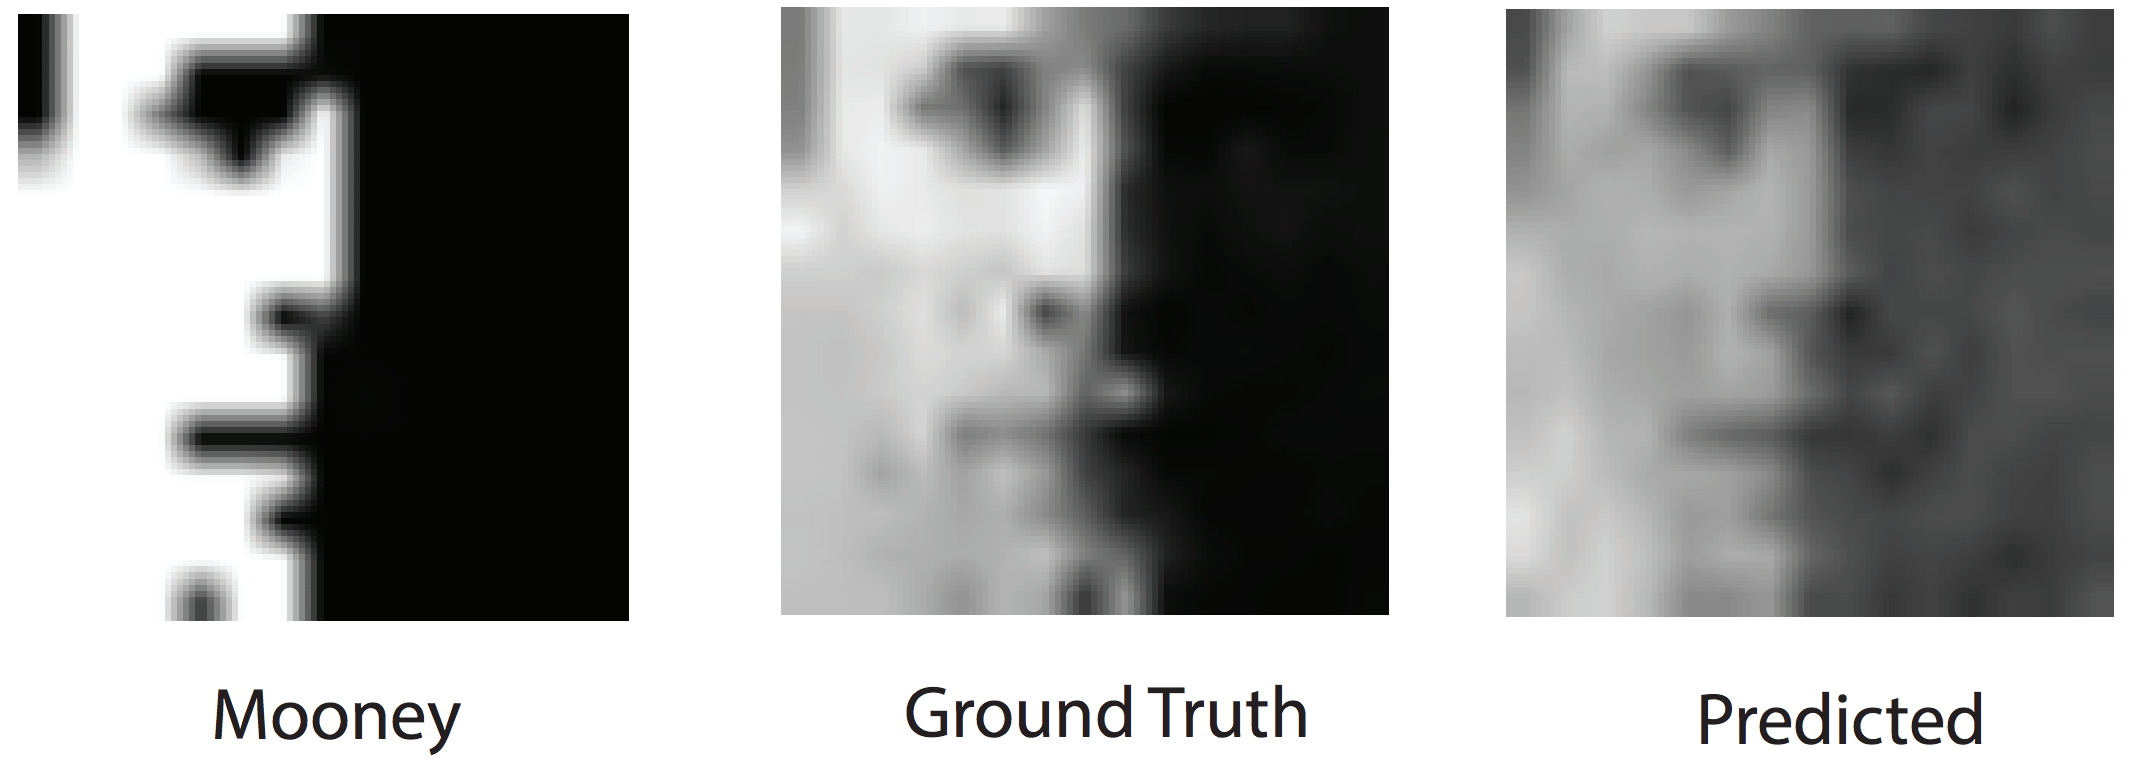
\includegraphics[scale=.4]{images/mooney_examples}    \caption{Example results with the input on the left and output on the right} \label{fig:robot}    \end{center} \end{figure}
\BeginSolution
%3e

\EndSolution
\end{enumerate}
%%%% Problem 3 Ends Here %%%%
\clearpage

%%%% Problem 4 Starts Here %%%%
\vspace{-2mm}\noindent\begin{mybox}{\begin{center}\textbf{\color{black}Problem 4: [Midterm] Bias-Variance for Ridge Regression \textit{(24 points)}}\end{center}}\end{mybox}\vspace{-2mm}
\vspace{10pt}
\noindent Consider the scalar data-generation model: \begin{align*}    Y = xw^* + Z\end{align*} where $x$ denotes the scalar input feature, $Y$ denotes the scalar noisy measurement, $Z \sim \mathcal{N}(0, 1)$ is standard unit-variance zero-mean Gaussian noise, and $w^*$ denotes the true generating parameter that we would like to estimate.
\vspace{4pt}

\noindent We are given a set of $n$ training samples $\{x_i, y_i\}_{i=1}^n$ that are generated by the above model with i.i.d.~$Z_i$ and distinct $x_i$. Our goal is to fit a linear model and get an estimate $\widehat{w}$ for the true parameter $w^*$. For all parts, assume that $x_i$'s are given and fixed (not random).
\vspace{4pt}

\noindent For a given training set $\{x_i, y_i\}_{i=1}^n$, the ridge-regression estimate for $w^*$ is defined by\begin{align*}     \whatridge     =\arg\min_{w \in \R} \, \lambda w^2 + \sum_{i=1}^n (y_i - x_i w)^2 \qquad\text{with $\lambda \geq 0.$} \end{align*} For the rest of the problem, assume that this has been solved and written in the form: \begin{align} \whatridge = \frac{S_{xy}}{s^2_{x}+\lambda} \end{align} where $S_{xy} = \sum_{i=1}^n x_i Y_i$ and $s_{x}^2 = \sum_{i=1}^n x_i^2$.
\vspace{4pt}

\noindent (This is given, no need to re-derive it).
\begin{enumerate}
\item (8 pts) {\bf Compute the squared-bias of the ridge estimate $\whatridge$ defined as follows}\begin{align}    \text{Bias}^2(\whatridge) &= (\ev[\whatridge] - w^*)^2. \label{eq:bias}    \end{align}It is fine if your answer depends on $w^*$ or $s_{x}$, but it should not depend directly or indirectly on the realizations of the random $Z$ noise. (So, no $S_{xy}$ allowed.)
\vspace{4pt}

\noindent {\em Hint: First compute the expectation of the estimate $\whatridge$ over the noises $Z$ in the observation.}
\BeginSolution
%4a

\EndSolution
\item (8 pts) {\bf Compute the variance of the estimate $\whatridge$ which is defined as}\begin{align}        \text{Var}(\whatridge) &= \ev[(\whatridge - \ev[\whatridge])^2]. \label{eq:var}\end{align}{\em Hint: It might be useful to write $\whatridge = \ev[\whatridge] + R$ for some random variable $R$.}
\BeginSolution
%4b

\EndSolution
\item (8 pts)  {\bf Describe how the squared-bias and variance of the estimate $\whatridge$ change as we change the value of $\lambda$? What happens as $\lambda \rightarrow 0$? $\lambda \rightarrow \infty$? Is the bias increasing or decreasing? Is the variance increasing or decreasing? In what sense is there a bias/variance tradeoff?}
\BeginSolution
%4c

\EndSolution
\end{enumerate}
%%%% Problem 4 Ends Here %%%%
\clearpage

%%%% Problem 5 Starts Here %%%%
\vspace{-2mm}\noindent\begin{mybox}{\begin{center}\textbf{\color{black}Problem 5: [Midterm] Hospital \textit{(25 points)}}\end{center}}\end{mybox}\vspace{-2mm}
\vspace{10pt}
\noindent You work at hospital A. Your hospital has collected patient data to build a model to predict who is likely to get sepsis (a bad outcome). Specifically, the data set contains the feature matrix $\X \in \R^{n \times d}$, and associated real number labels $\y \in \R ^ n$, where $n$ is the number of patients you are learning from and $d$ is the number of features describing each patient. You plan to fit a linear regression model $\widehat{y} = \w^{\top} \vec{x}$ that will enable you to predict a label for future, unseen patients (using their feature vectors).
\vspace{4pt}

\noindent However, your hospital has only started collecting data a short time ago. Consequently the model you fit is not likely to be particularly accurate. Hospital B has exactly the same set up as your hospital (i.e., their patients are drawn from the same distribution as yours and they have the same measurement tools). For privacy reasons, Hospital B will not share their data. However, they tell you that they have trained a linear model on their own sepsis-relevant data: ($\X_B$ and $\y_B$) and are willing to share their learned model $\widehat{y} = \w_B^{\top} \vec{x}$ with you. In particular, Hospital B shares their entire Gaussian posterior distribution on $\w$ with you: $\calN(\w_B, \Psi)$.
\begin{enumerate}
\item (10 pts) Assume that we use the posterior from Hospital B as our own prior distribution for $\w \sim \calN(\w_B, \Psi)$. Suppose that our Hospital A model is given by $\y = \X \w + \vec{\epsilon}$, where the noise, $\vec{\epsilon}$, has an assumed distribution $\vec{\epsilon} \sim \calN(0, \I)$. \textbf{Derive the MAP estimate $\widehat{\w}$ for $\w$ using Hospital A's data $\X, \y$ and the prior information from Hospital B.}
\vspace{4pt}

\noindent {\em HINT: Recall that traditional ridge regression could be derived from a MAP perspective, where the parameter $\w$ has a zero mean Gaussian prior distribution with a scaled identity covariance. How could you use reparameterization (i.e.~change of variables) for the problem here?}
\BeginSolution
%5a

\EndSolution
\item (15 pts) Now, for simplicity, consider $d=1$ so that the $w$ is a scalar parameter. Suppose that instead of giving you their posterior distribution, Hospital B only gave you their mean $\widehat{w}_B$. How can you use this information to help fit your model? \textbf{Describe in detail how you should use your own hospital's patient data and combine it with the mean $\widehat{w}_B$ from Hospital B in a procedure to find your own $\widehat{w}$ for predicting sepsis in Hospital A.}
\vspace{4pt}

\noindent {\em Hint 1: You might want to consider introducing an appropriate hyperparameter and doing what you usually do with hyperparameters. }
\vspace{4pt}

\noindent {\em Hint 2: What does the $\lambda$ hyperparameter in ridge-regression correspond to from a probabilistic perspective?}
\BeginSolution
%5b

\EndSolution
\end{enumerate}
%%%% Problem 5 Ends Here %%%%
\clearpage

%%%% Problem 6 Starts Here %%%%
\vspace{-2mm}\noindent\begin{mybox}{\begin{center}\textbf{\color{black}Problem 6: [Midterm] Ridge regression vs. PCA \textit{(24 points)}}\end{center}}\end{mybox}\vspace{-2mm}
\vspace{10pt}
\noindent Assume we are given $n$ training data points $(\vec{x}_i, y_i)$. We collect the target values into $\vec{y} \in \R^n$, and the inputs into the matrix $\mat{X} \in \R^{n\times d}$ where the rows are the $d-$dimensional feature vectors $\vec x_i^\top$ corresponding to each training point. Furthermore, assume that $\frac{1}{n}\sum_{i=1}^n\vec{x_i} = \vec{0}$, $n > d$ and $\mat{X}$ has rank $d$.
\vspace{4pt}

\noindent In this problem we want to compare two procedures: The first is ridge regression with hyperparameter $\lambda$, while the second is applying ordinary least squares after using PCA to reduce the feature dimension from $d$ to $k$ (we give this latter approach the short-hand name $k$-PCA-OLS where $k$ is the hyperparameter).
\vspace{4pt}

\noindent Notation: The singular value decomposition of $\mat{X}$ reads $\mat{X} = \mat{U} \mat{\Sigma} \mat{V}^\top$ where $\mat{U} \in \R^{n\times n}$, $\mat{\Sigma} \in \R^{n\times d}$ and $\mat{V} \in \R^{d\times d}$. We denote by $\vec{u}_i$ the $n$-dimensional column vectors of $\mat{U}$ and by $\vec{v}_i$ the $d-$dimensional column vectors of $\mat{V}$. Furthermore the diagonal entries $\sigma_i = \Sigma_{i,i}$ of $\mat \Sigma$ satisfy $\sigma_1 \geq \sigma_2 \geq \dots \geq \sigma_d > 0$. For notational convenience, assume that $\sigma_i = 0$ for $i > d$.
\begin{enumerate}
\item (6 pts) It turns out that the ridge regression optimizer (with $\lambda
> 0$) in the $\mat{V}$-transformed coordinates
    \begin{equation*}
    \hatwridge = \arg \min_{\vec{w}} \| \mat{X} \mat{V} \vec{w} - \vec{y}\|_2^2 + \lambda \| \vec{w}\|_2^2
    \end{equation*}
    has the following expression:
    \begin{equation} \label{eq:ridgevector}
      \hatwridge = \diag\left(\frac{\sigma_i}{\lambda + \sigma_i^2}\right) \mat{U}^\top \vec{y}.
    \end{equation}
        
    Use $\widehat{y}_{test} = \vec{x}_{test}^{\top} \mat{V} \hatwridge$ to denote the resulting prediction for a
    hypothetical $\vec{x}_{test}$. Using \eqref{eq:ridgevector} and
    the appropriate $\{\beta_i\}$, this can be written as:
\begin{equation}
\label{eq:pred}
\widehat{y}_{test} = \vec{x}_{test}^\top \sum_{i=1}^d \vec{v}_i \beta_i \vec{u}_i^\top \vec{y}.
\end{equation}
{\bf What are the $\beta_i$ for this to correspond to \eqref{eq:ridgevector} from ridge regression?}
\BeginSolution
%6a

\EndSolution
\item (12 pts) Suppose that we do k-PCA-OLS --- i.e.~ordinary least squares on the reduced $k$-dimensional feature space obtained by projecting the raw feature vectors onto the $k < d$ principal components of the covariance matrix $\mat{X}^\top \mat{X}$. Use $\widehat{y}_{test}$ to denote the resulting prediction for a hypothetical $\vec{x}_{test}$,
\vspace{4pt}

\noindent It turns out that the learned k-PCA-OLS predictor can be written as: \begin{equation} \label{eq:pred}\widehat{y}_{test} = \vec{x}_{test}^\top \sum_{i=1}^d \vec{v}_i \beta_i \vec{u}_i^\top \vec{y}. \end{equation} {\bf Give the $\beta_i$ coefficients for k-PCA-OLS. Show work.}
\vspace{4pt}

\noindent {\em Hint 1: some of these $\beta_i$ will be zero. Also, if you want to use the compact form of the SVD, feel free to do so if that speeds up your derivation.
\vspace{4pt}

\noindent Hint 2: some inspiration may be possible by looking at the next partfor an implicit clue as to what the answer might be.}
\BeginSolution
%6b

\EndSolution
\item (6 pts) For the following part, $d=5$. The following $\vec{\beta}:=(\beta_1,\ldots,\beta_{5})$  (written out to two significant figures) are the results of OLS (i.e.~what we would get from ridge regression in the limit $\lambda \rightarrow 0$), $\lambda$-ridge-regression, and $k$-PCA-OLS for some $\mat{X},\vec{y}$ (identical for each method) and $\lambda=1, k=3$. {\bf Write down which procedure was used for each of the three sub-parts below.}
\vspace{4pt}

\noindent We hope this helps you intuitively see the connection between these three methods.
\vspace{4pt}

\noindent {\em Hint: It is not necessary to find the singular values of $\mat{X}$ explicitly, or to do any numerical computations at all.}
\begin{enumerate}[i.]
\item $\vec{\beta} = (0.01, 0.1, 0.5, 0.1, 0.01)$
\BeginSolution
%6ci

\EndSolution
\item $\vec{\beta} =  (0.01, 0.1, 1, 0, 0)$
\BeginSolution
%6cii

\EndSolution
\item $\vec{\beta} =  (0.01, 0.1, 1, 10, 100)$
\BeginSolution
%6ciii

\EndSolution
\end{enumerate}
\end{enumerate}
%%%% Problem 6 Ends Here %%%%
\clearpage

%%%% Problem 7 Starts Here %%%%
\vspace{-2mm}\noindent\begin{mybox}{\begin{center}\textbf{\color{black}Problem 7: [Midterm] Kernel PCA \textit{(24 points)}}\end{center}}\end{mybox}\vspace{-2mm}
\vspace{10pt}
\noindent In lectures, discussion, and homework, we learned how to use PCA to do dimensionality reduction by projecting the data to a subspace that captures most of the variability. This works well for data that is roughly Gaussian shaped, but many real-world high dimensional datasets have underlying low-dimensional structure that is not well captured by linear subspaces. However, when we lift the raw data into a higher-dimensional feature space by means of a nonlinear transformation, the underlying low-dimensional structure once again can manifest as an approximate subspace. Linear dimensionality reduction can then proceed. As we have seen in class so far, kernels are an alternate way to deal with these kinds of nonlinear patterns without having to explicitly deal with the augmented feature space. This problem asks you to discover how to apply the ``kernel trick'' to PCA.
\vspace{4pt}

\noindent Let $\X \in \R^{n \times \ell}$ be the data matrix, where $n$ is the number of samples and $\ell$ is the dimension of the raw data. Namely, the data matrix contains the data points $\vec x_j \in \R^\ell$ as rows \begin{align}\X = \begin{pmatrix}\vec x_1^\top\\\vec x_2^\top\\\vdots\\\vec x_n^\top\end{pmatrix}\in \R^{n\times \ell}.\end{align}
\begin{enumerate}
\item (5 pts) \textbf{Compute $\X \X^\top$ in terms of the singular value decomposition $\mat X = \mat U\mat \Sigma \mat V^\top$ where $\mat U \in \R^{n\times n}, \mat \Sigma \in \R^{n\times \ell}$ and $\vec V \in \R^{\ell \times \ell}$.} Notice that $\X \X^\top$ is the matrix of pairwise Euclidean inner products for the data points. \textbf{How would you get $\mat U$ if you only had access to $\X \X^\top$?}
\BeginSolution
%7a

\EndSolution
\item (7 pts) Given a new test point $\vec x_{test} \in \R^{\ell}$, one central use of PCA is to compute the projection of $\vec x_{test}$ onto the subspace spanned by the $k$ top singular vectors $\vec v_1, \vec v_2, \ldots, \vec v_k$.
\vspace{4pt}

\noindent \textbf{Express the scalar projection $z_j = \vec v_j^\top \vec x_{test}$ onto the $j$-th principal component  as a function of the inner products}\begin{align}\mat X \vec x_{test} =\begin{pmatrix}  \langle \vec x_1, \vec x_{test}\rangle\\  \vdots\\  \langle \vec x_n, \vec x_{test}\rangle\end{pmatrix}.\end{align}
\vspace{4pt}

\noindent Assume that all diagonal entries of $\mat \Sigma$ are nonzero and non-increasing, that is $\sigma_1 \geq \sigma_{2} \geq \cdots > 0$.
\vspace{4pt}

\noindent {\em Hint: Express $\mat V^\top$ in terms of the singular values $\mat \Sigma$, the left singular vectors $\mat U$ and the data matrix $\mat X$. If you want to use the compact form of the SVD, feel free to do so.}
\BeginSolution
%7b

\EndSolution
\item (12 pts) How would you define kernelized PCA for a general kernel function $k(\vec x_i, \vec x_j)$ (to replace the Euclidean inner product $\langle \vec x_i, \vec x_j\rangle$)? For example, the RBF kernel $k(\vec x_i, \vec x_j) = \exp(-\frac{\|\vec x_i  - \vec  x_j\|^2}{\delta^2})$.
\vspace{4pt}

\noindent {\bf Describe this in terms of a procedure which takes as inputs the training data points $\vec x_1, \vec x_2, \ldots, \vec x_n \in \R^\ell$ and the new test point $\vec x_{test}\in \R^\ell$, and outputs the analog of the previous part's $z_j$ coordinate in the kernelized PCA setting. You should include how to compute $\mat U$ from the data, as well as how to compute the analog of $\mat X \vec x_{test}$ from the previous part.}
\vspace{4pt}

\noindent Invoking the SVD or computing eigenvalues/eigenvectors is fine in your procedure, as long as it is clear what matrix is having its SVD or eigenvalues/eigenvectors computed. The kernel $k(\cdot, \cdot)$ can be used as a black-box function in your procedure as long as it is clear what arguments it is being given.
\BeginSolution
%7c

\EndSolution
\end{enumerate}
%%%% Problem 7 Ends Here %%%%
\clearpage

%%%% Problem 8 Starts Here %%%%
\vspace{-2mm}\noindent\begin{mybox}{\begin{center}\textbf{\color{black}Problem 8: [Midterm] Multiple Choice Questions \textit{(14 points)}}\end{center}}\end{mybox}\vspace{-2mm}
\vspace{10pt}
\noindent For these questions, select \underline{\bf all} the answers which are correct. You will get full credit for selecting all the right answers. On some questions, real-valued partial credit will be assigned. You will be graded on your {\bf best seven of nine, so feel free to skip up to two of them.}
\begin{enumerate}
\item Let $\mat{X} \in \mathbb{R}^{n \times d} $ with $n \geq d$. Suppose $\mat{X} = \mat{U}${\boldmath$\Sigma$}$\mat{V}^\top$ is the singular value decomposition of $\mat X$ where $\sigma_i = \Sigma_{i,i}$ are the diagonal entries of $\mat \Sigma$ and satisfy $\sigma_1 \geq \sigma_2\geq \dots \geq \sigma_d$ while $\vec{u}_i$ and $\vec{v}_i$ are the ith columns of $\mat{U}$ and $\mat{V}$ respectively.  {\bf Which of the following is the rank $k$ approximation to $\mat{X}$ that is best in the Froebenius norm.} That is, which low rank approximation, $\mat{X}_k$, for $\mat{X}$ yields the lowest value for $\lvert\lvert\mat{X}-\mat{X}_k\rvert\rvert^2_F$? \begin{multicols}{4}\begin{itemize}[label=(\Alph*)]\citem $\sum_{i=1}^k \sigma_i \vec{u}_i \vec{v}_{n-i}^\top$\citem $\sum_{i=1}^k \sigma_i \vec{u}_i \vec{v}_{i}^\top$\citem $\sum_{i=d-k+1}^d \sigma_i \vec{u}_i \vec{v}_{i}^\top$\citem $\sum_{i=1}^k \sigma_i \vec{u}_{n-i} \vec{v}_{i}^\top$\end{itemize}\end{multicols}
\BeginSolution
%8a

\EndSolution
\item Consider a simple dataset of points $(x_i, y_i) \in \R^2$, each associated with a label $b_i$ which is $-1$ or $+1$. The dataset was generated by sampling data points with label $-1$ from a disk of radius $1.0$ (shown as filled circles in the figure) and data points with label $+1$ from a ring with inner radius $0.8$ and outer radius $2.0$ (shown as crosses in the figure). {\bf Which set of polynomial features would be best for performing linear regression, assuming at least as much data as shown in the figure?}
\begin{center}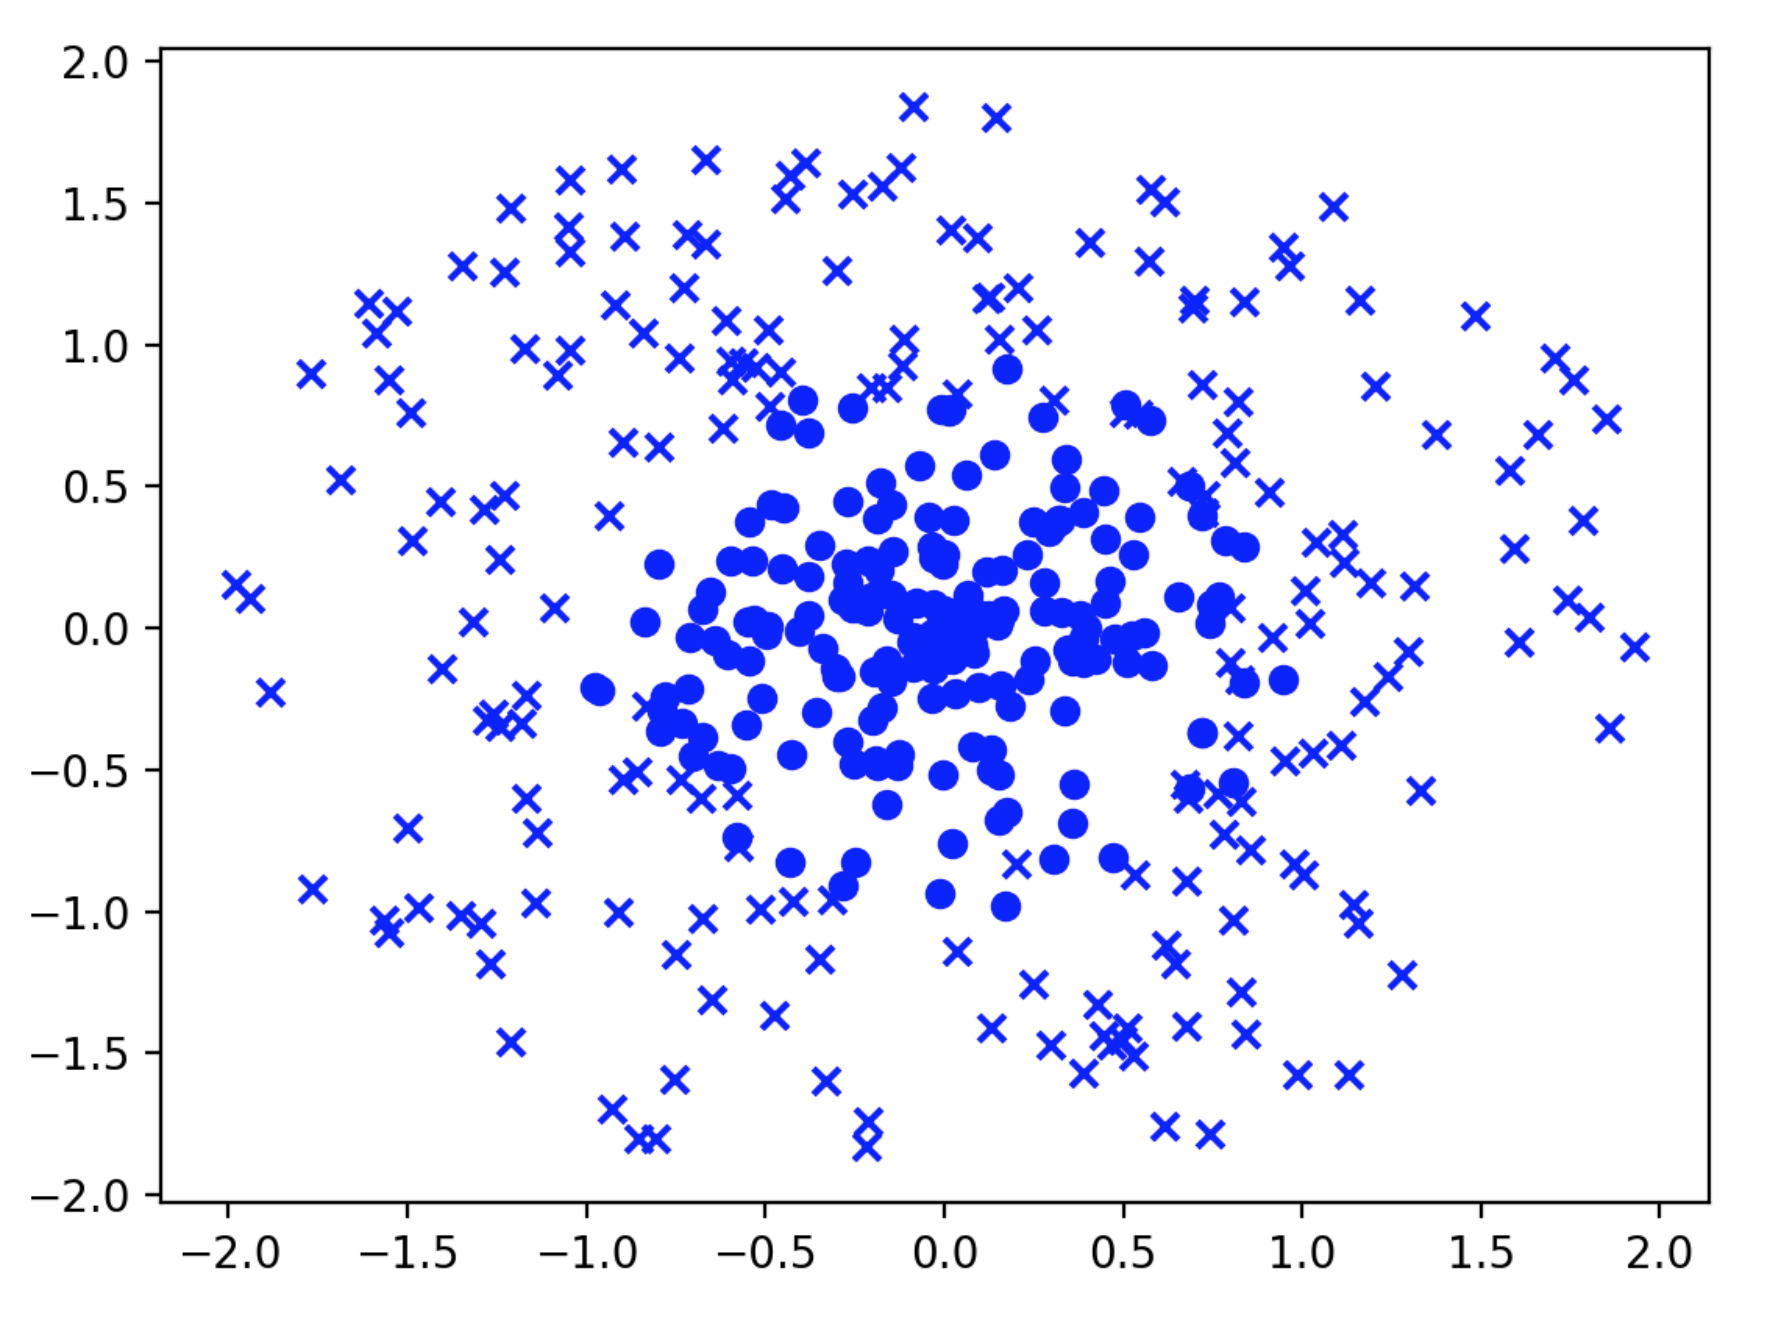
\includegraphics[width=0.8\textwidth]{images/b}\end{center}\begin{multicols}{2}\begin{itemize}\citem $1, x_i$\citem $1, x_i, y_i$\citem $1, x_i, y_i, x_i^2, x_iy_i, y_i^2$\citem $1, x_i, y_i, x_i^2, x_iy_i, y_i^2, x_i^3, y_i^3, x_i^2y_i, x_iy_i^2$\end{itemize}\end{multicols}
\BeginSolution
%8b

\EndSolution
\item {\bf Which of the following is a valid kernel function} for vectors of the same length, $\vec{x}$ and $\vec{y}$? \begin{multicols}{2}\begin{itemize}\citem  $k(\vec{x}, \vec{y}) = \vec{x}^\top \vec{y}$\citem  $k(\vec{x}, \vec{y}) = e^{-\frac{1}{2} \lvert\lvert \vec{x} - \vec{y} \rvert\rvert^2_2}$\citem  $k(\vec{x}, \vec{y}) = (1+\vec{x}^\top \vec y)^p$ for some degree p\citem  $k(\vec{x}, \vec{y}) = k_1(\vec x,\vec y) - k_2(\vec x,\vec y)$ for valid kernels $k_1$ and $k_2$.\end{itemize}\end{multicols}
\BeginSolution
%8c

\EndSolution
\item During training of your model, both independent variables in the matrix $\mat X\in \R^{n\times d}$ and dependent target variables $\vec y\in \R^n$ are corrupted by noise. At test time, the data points you are computing predictions for, $\vec x_{test}$, are noiseless. {\bf Which method(s) should you use to estimate the value of $\vec{\hat{w}}$ from the training data in order to make the most accurate predictions $\vec y_{test}$ from the noiseless test input data, $\mat X_{test}$?} Assume that you make predictions using $\vec y_{test}=\mat X_{test} \vec{\hat{w}}$. \begin{multicols}{2}\begin{itemize}\citem  OLS\citem  Ridge regression\citem  Weighted Least Squares\citem  TLS\end{itemize}\end{multicols}
\BeginSolution
%8d

\EndSolution
\item Assume you have $n$ input data points, each with $d$ high quality features ($\mat X\in \R^{n\times d}$) and associated labels ($\vec y\in \R^n$). Suppose that $d \gg n$ and that you want to learn a linear predictor. {\bf Which of these approaches would help you to avoid overfitting?} \begin{multicols}{2}\begin{itemize}\citem  Preprocess $\mat X$ using $k \ll n$ random projections \citem  Preprocess $\mat X$ using PCA with $k \ll n$ components.\citem  Preprocess $\mat X$ using PCA with $n$ components.\citem  Add polynomial features\citem  Use a kernel approach \citem  Add a ridge penalty to OLS \citem  Do weighted least squares\end{itemize}\end{multicols}
\BeginSolution
%8e

\EndSolution
\item {\bf Which methods could yield a transformation to go from the two-dimensional data on the left to the two-dimensional data on the right? }\begin{center} 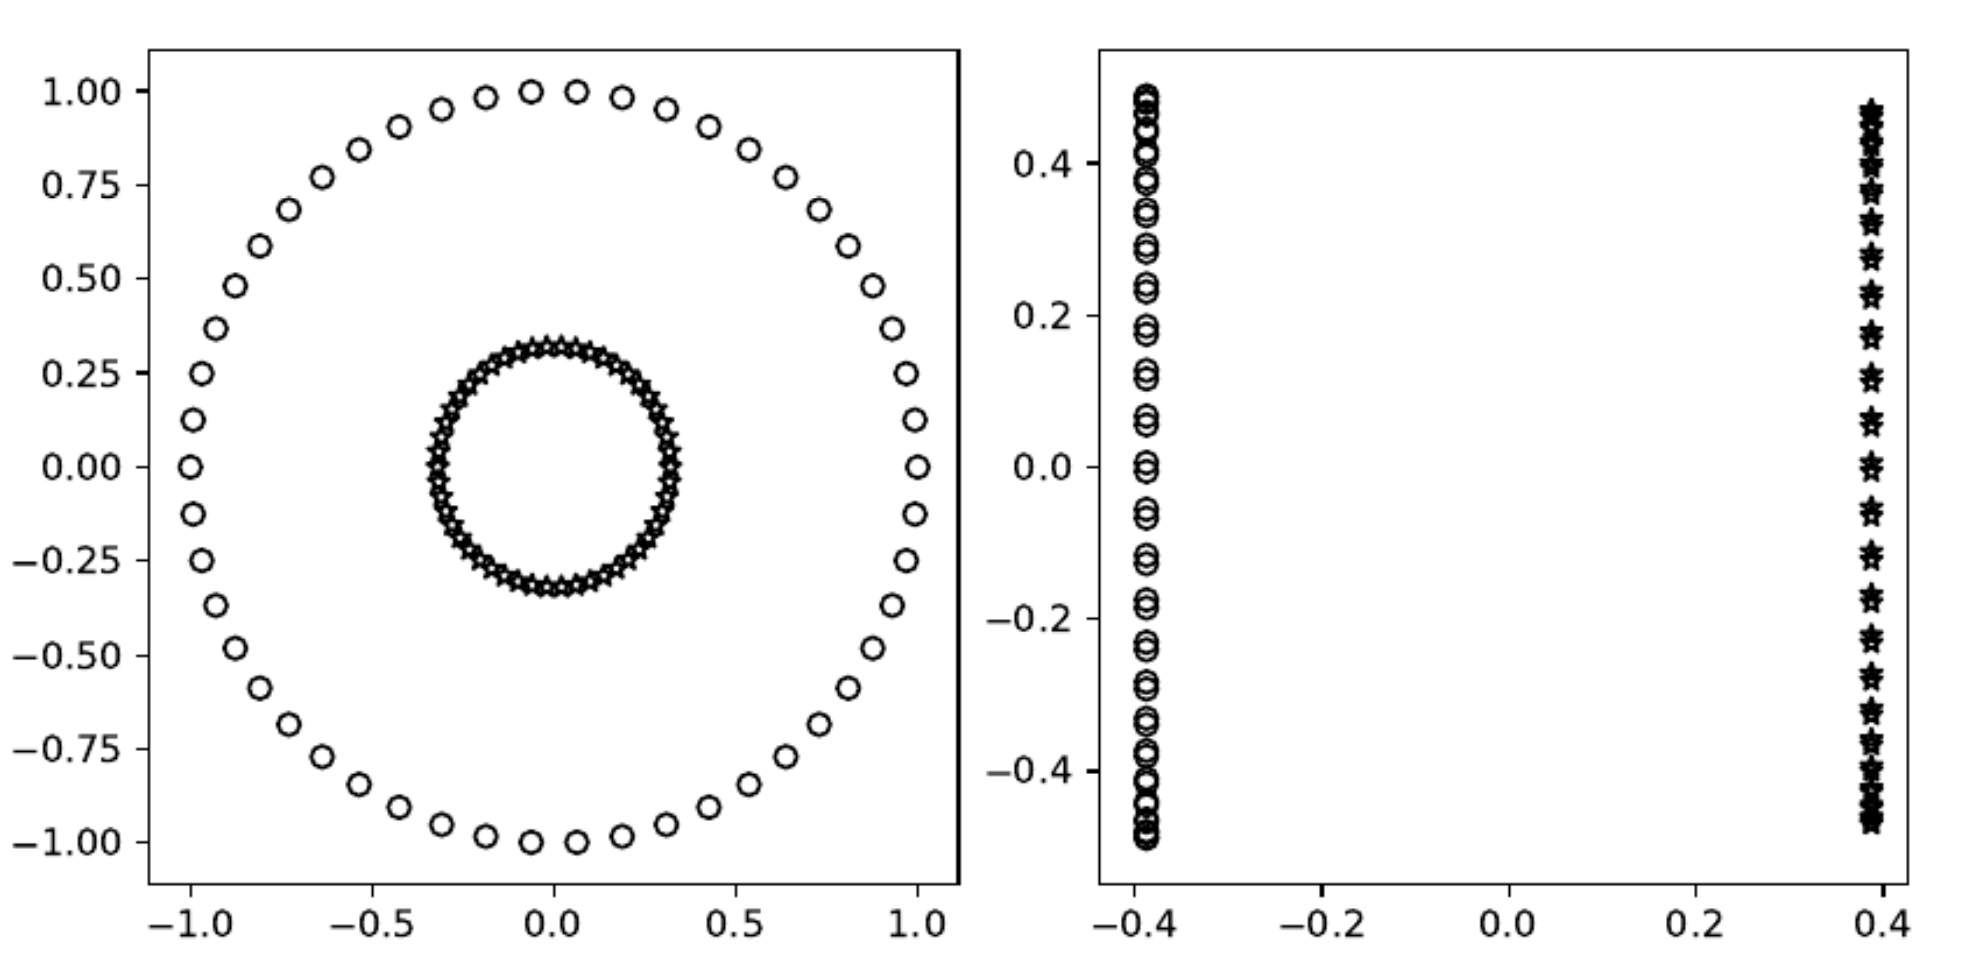
\includegraphics[width=.8\linewidth]{images/f} \end{center}\begin{multicols}{2}\begin{itemize}\citem  Random projections\citem  PCA\citem  Use of a kernel\citem  Adding polynomial features\end{itemize}\end{multicols}
\BeginSolution
%8f

\EndSolution
\item Your friend is training a machine learning model to predict disease severity based on $k$ different health indicators. She generates the following plot, where the value of $k$ is on the $x$ axis. \begin{align*}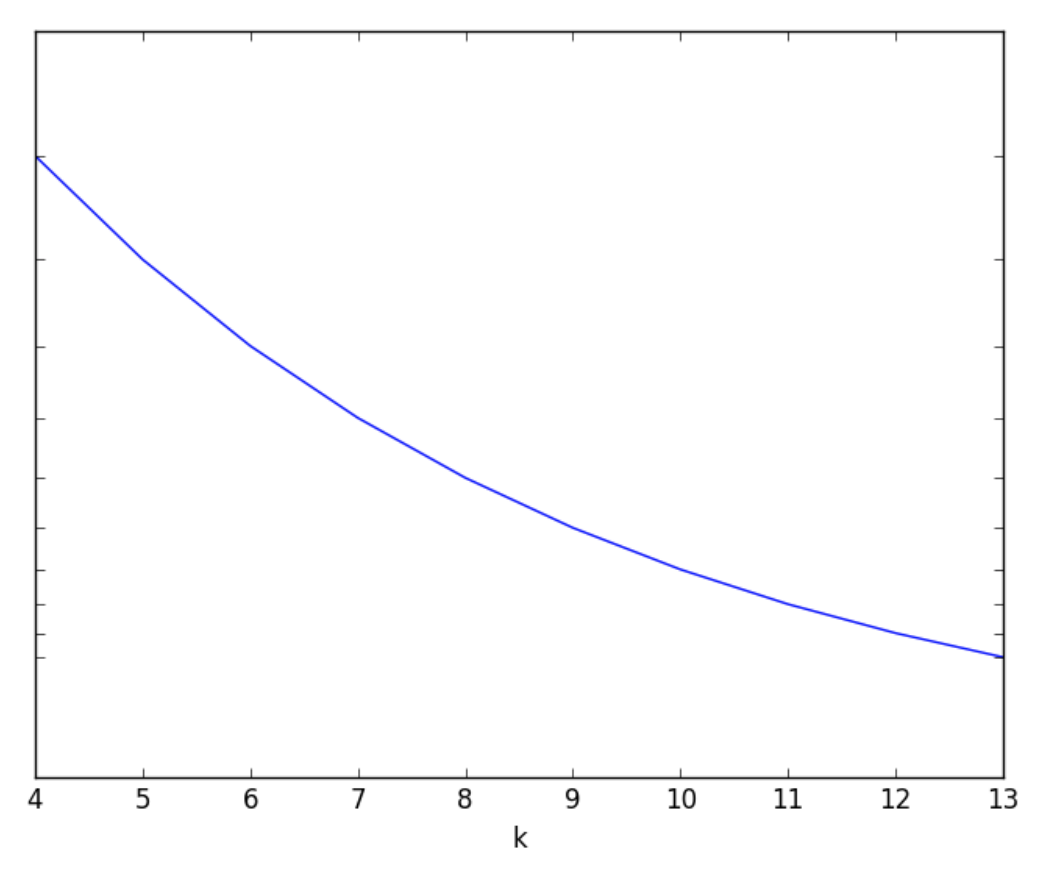
\includegraphics[width=0.5\textwidth]{images/g}\end{align*}{\bf Which of these might the $y$ axis represent?}\begin{multicols}{2}\begin{itemize}\citem Training Error\citem Validation Error\citem Bias\citem Variance\end{itemize}\end{multicols}
\BeginSolution
%8g

\EndSolution
\item Your friend is training a machine learning model to predict disease severity based on $k$ different health indicators. She generates the following plot, where the value of $k$ is on the $x$ axis. \begin{align*}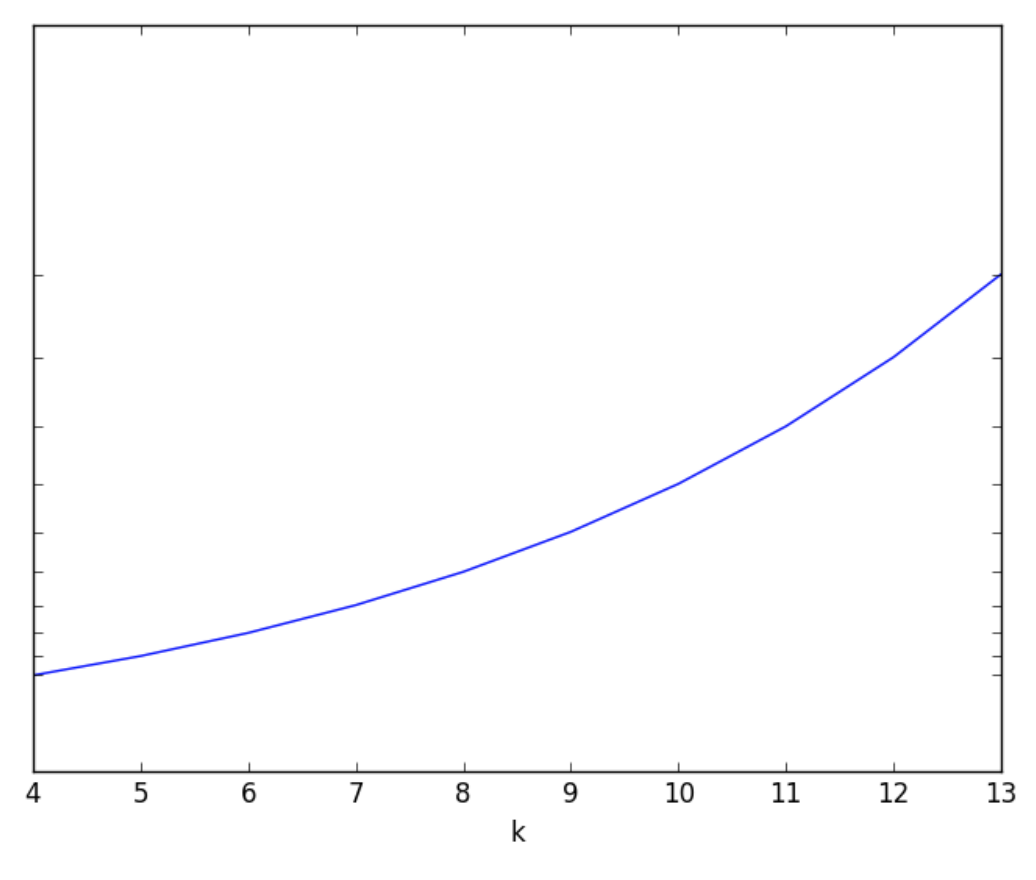
\includegraphics[width=0.5\textwidth]{images/h}\end{align*}{\bf Which of these might the $y$ axis represent?}\begin{multicols}{2}\begin{itemize}\citem Training Error\citem Validation Error\citem Bias\citem Variance\end{itemize}\end{multicols}
\BeginSolution
%8h

\EndSolution
\item Your friend is training a machine learning model to predict disease severity based on $k$ different health indicators. She generates the following plot, where the value of $k$ is on the $x$ axis.\begin{align*}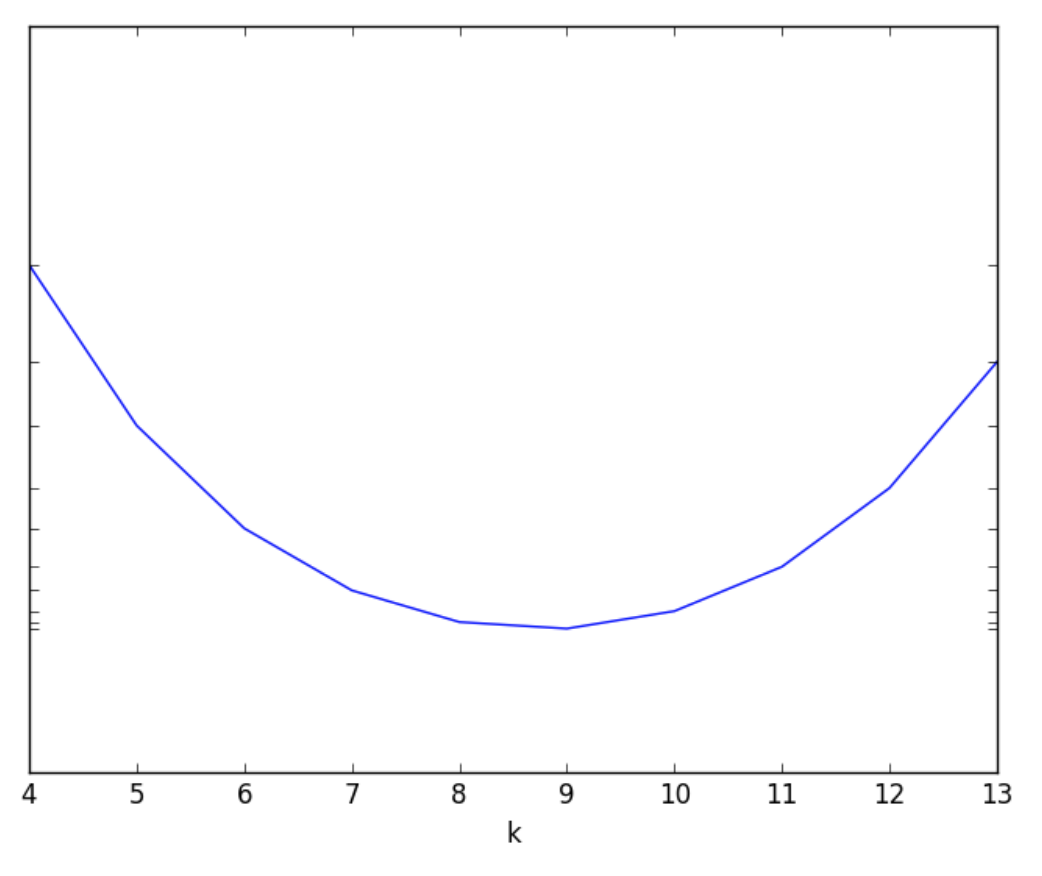
\includegraphics[width=0.5\textwidth]{images/i}\end{align*}{\bf Which of these might the $y$ axis represent?}\begin{multicols}{2}\begin{itemize}\citem  Training Error\citem  Validation Error\citem  Bias\citem Variance\end{itemize}\end{multicols}
\BeginSolution
%8i

\EndSolution
\end{enumerate}
%%%% Problem 8 Ends Here %%%%
\clearpage

%%%% Problem 9 Starts Here %%%%
\vspace{-2mm}\noindent\begin{mybox}{\begin{center}\textbf{\color{black}Problem 9: Your Own Question}\end{center}}\end{mybox}\vspace{-2mm}
\vspace{10pt}
\noindent \textbf{Write your own question, and provide a thorough solution.}
\vspace{3pt}

\noindent Writing your own problems is a very important way to really learn the material. The famous ``Bloom's Taxonomy'' that lists the levels of learning is: Remember, Understand, Apply, Analyze, Evaluate, and Create. Using what you know to create is the top-level. We rarely ask you any HW questions about the lowest level of straight-up remembering, expecting you to be able to do that yourself. (e.g. make yourself flashcards) But we don't want the same to be true about the highest level.
\vspace{3pt}

\noindent As a practical matter, having some practice at trying to create problems helps you study for exams much better than simply counting on solving existing practice problems. This is because thinking about how to create an interesting problem forces you to really look at the material from the perspective of those who are going to create the exams. 
\vspace{3pt}

\noindent Besides, this is fun. If you want to make a boring problem, go ahead. That is your prerogative. But it is more fun to really engage with the material, discover something interesting, and then come up with a problem that walks others down a journey that lets them share your discovery. You don't have to achieve this every week. But unless you try every week, it probably won't happen ever. 
\BeginSolution
%5

\EndSolution
%%%% Problem 9 Ends Here %%%%
\clearpage

%%%% Code Appendix Starts Here %%%%
\vspace{-2mm}\noindent\begin{mybox}{\begin{center}\textbf{\color{black}Code Appendix}\end{center}}\end{mybox}\vspace{-2mm}
\begin{itemize}
\item \texttt{mooney\_starter.py}
\BeginSolution
% Paste Code Between Verbatim
\begin{verbatim}

\end{verbatim}
\EndSolution
\end{itemize}
%%%% Code Appendix Ends Here %%%%

\end{document}
%%%%% Template Ends Here %%%%%